\chapter{Cross-loop Optimization of Arithmetic Intensity for Finite Element Integration}
\label{ch:lowlevelopt}

In the previous chapter, a method to minimize the operation count of finite element integration loop nests, or ``assembly kernels'', has been developed. Here, the focus is on the same class of kernels, but a complementary issue is tackled: the low level optimization of the resulting code. 

This chapter is partly extracted from \cite{Luporini-coffee}.

\section{Recapitulation and Objectives}

We know that an assembly kernel is characterized by the presence of an affine, often non-perfect loop nest, in which individual loops are rather small: their trip count rarely exceeds 30, and may be as low as 3 for low order methods. In the innermost loop, a compute intensive expression evaluates an $n$-dimensional array, or element tensor, which represents the result of local assembly in an element of the discretized domain. More specifically: in bilinear forms, $n=2$ and the output is referred to as element matrix; in linear forms, $n=1$ and the output is referred to as element vector. With such a kernel structure, the objective of the low level optimization is maximizing register locality and SIMD vectorization.

We aim to maximize our impact on the platforms that are realistically used for finite element applications, so we target conventional CPU architectures rather than GPUs. The key limiting factor to the execution on GPUs is the stringent memory requirements. Only relatively small problems fit in a GPU memory, and support for distributed GPU execution in general purpose finite element frameworks is minimal. There has been some research on adapting local assembly to GPUs, although it differs from ours in several ways, including: (i) not relying on automated code generation from a domain-specific language, (ii) testing only very low order methods, (iii) not optimizing for cross-loop arithmetic intensity (the goal is rather effective multi-thread parallelization). In addition, our code transformations would drastically impact the GPU parallelization strategy, for example by increasing a thread's working set. For all these reasons, a study on extending the research to GPU architectures is beyond the scope of this work. The related work on the subject is covered in Section~\ref{sec:coffee-related-work}, while intuitions about this research direction are provided in Section~\ref{sec:generality}.

Achieving high-performance on CPUs is non-trivial. The complexity of the mathematical expressions, which we know to be often characterized by a large number of operations on constants and small vectors, makes it hard to determine a single or specific sequence of transformations that is successfully applicable to all problems. Loop trip counts are typically small and can vary significantly, which further exacerbates the issue. Moreover, the memory access pattern can be either unit-stride (\texttt{A[i]}, \texttt{A[i+1]}, \texttt{A[i+2]}, ...) or multi-stride (\texttt{A[i]}, \texttt{A[i+1]}, \texttt{A[i+N]}, \texttt{A[i+N+1]}, ...) -- for example, as a consequence of skipping useless floating-point operations, see Section~\ref{sec:zeros}. We will show that general-purpose compilers, such as \emph{GNU's} and \emph{Intel's}, fail at maximizing the efficiency of the generated code because of such a particular structure. Polyhedral-model-based source-to-source compilers, for instance~\cite{pluto}, can apply aggressive loop optimizations, such as tiling, but these are not particularly helpful in our context since they mostly focus on cache locality. 

As in Chapter~\ref{ch:optimality}, we focus on optimizing the performance of assembly kernels produced through automated code generation, so we seek transformations that are generally applicable and effective. In particular, we introduce and study the following transformations:

\begin{description}
\item[Padding and data alignment] SIMD vectorization is more effective when the CPU registers are packed (unpacked) by means of aligned load (store) instructions. Data alignment is achieved through array padding, a conceptually simple yet powerful transformation that can result in dramatic reductions in execution time. 
\item[Vector-register tiling] Tiling at the level of vector registers exploits the peculiar memory access pattern induced by finite element operators (i.e., the linearity of the test and trial functions loops) to improve data locality.
\item[Expression splitting] Complex expressions are often characterized by high register pressure (i.e., the lack of available registers inducing the compiler to ``spill'' data from registers to cache). This transformation exploits the associativity property of the addition to distribute, or ``split'', an expression into multiple sub-expressions to be computed in separate loop nests.
\end{description}

In addition, we analyze the effects of ``more traditional'' optimizations: loop unroll, loop interchange, loop fusion and vector promotion. Some of these are not applied by general-purpose compilers, or are applied in a sub-optimal way; in such a case, they will be applied explicitly through our compiler, COFFEE. 

To summarize, the contributions of this chapter are:
\begin{itemize}
\item The introduction of novel transformations that are demonstrated to improve the performance of assembly kernels. These transformations, implemented in COFFEE, aim to maximize register locality and SIMD vectorization.
\item A study on the effectiveness of a set of well-known transformations as well as the introduction of extensions that, taking advantage of assembly kernel properties, maximize their impact.
\item Extensive experimentation using a set of real-world forms commonly arising in finite element methods.
\item A discussion concerning the generality of the transformations and their applicability to different domains.
\end{itemize}

\section{Low-level Optimization}
\label{sec:lowlevelopt}

In this section, we describe three novel transformations that target register locality (expression splitting), SIMD vectorization (padding and data alignment), or both (vector-register tiling). Their ideation was directly inspired by the structure of assembly kernels. In particular, preliminary experimentation and profiling suggested that better performance could be achieved by optimizing resource usage within a CPU core. The implementation is carried out in COFFEE. Understanding the potential of these transformations in other computational domains requires a different kind of investigation, which we approach in Section~\ref{sec:generality}. 

\subsection{Padding and Data Alignment}
\label{sec:coffee-padding}
The absence of stencils makes it simple for a general-purpose compiler to auto-vectorize the computation of the element tensor\footnote{In practice, the {\em GCC} compiler does not to auto-vectorize loops if these are too small; this indicates flaws in its cost model, since vectorization, in our hand-crafted experiments, was always found to be a winning choice.}. Nevertheless, vectorization is sub-optimal if data are not aligned to cache-line boundaries or if the innermost loop trip count is not a multiple of the vector length $\mbox{\texttt{VL}}$ (especially when the loops are small as in assembly kernels). 

Data alignment is enforced in two steps. First, all arrays (except the element tensor, for reasons discussed shortly) are allocated to addresses that are multiples of $\mbox{\texttt{VL}}$. This is achieved by adding special attributes to each declaration (e.g., {\tt $\_\_$attribute$\_\_$(aligned($\mbox{\texttt{VL}}*8$))}, with $8$ being the size of a value in double precision). Second, their innermost dimension is padded by rounding the size to the nearest multiple of $\mbox{\texttt{VL}}$. For instance, assume the original size of a basis function array is 3$\times$3 and $\mbox{\texttt{VL}}=4$ (e.g. AVX processor, with 32-byte long vector registers and 8-byte double-precision floats); then, the padded version of the array will have size 3$\times$4. The compiler is explicitly informed about data alignment through suitable pragmas. For example, in the case of the Intel compiler, adding the annotation \texttt{$\#$pragma vector aligned} to a loop declares that all of the memory accesses performed in its body will be aligned. This allows the compiler to generate aligned load and store instructions (e.g., {\tt movapd}), which are dramatically faster than unaligned ones (e.g., {\tt movupd}).

As anticipated, the element tensor requires special attention. In our computational model, the element tensor is a kernel's input parameter, so the aforementioned transformations cannot be applied. We therefore create a ``shadow'' copy of the element tensor, padded, aligned, and initialized to 0. The shadow element tensor replaces any occurrence of the original element tensor in the kernel. Right before returning to the caller, a loop nest willy copy the relevant region of the shadow element tensor back into the input array.

This process often allows to safely round a loop trip count to the nearest multiple of $\mbox{\texttt{VL}}$, thus avoiding the introduction of a remainder (scalar) loop from the compiler (which would render vectorization less efficient). We distinguish two cases:

\begin{description}
\item[All memory accesses in the kernel are unit-stride] It is trivial to verify whether the iterations introduced by rounding up the loop trip count will only write to the padded region of the element tensor. In such a case, the loop trip count can be rounded. Listing~\ref{code:weighted-laplace-licm-pad} illustrates the effect of padding and data alignment on top of generalized code motion in the weighted Laplace kernel which we introduced in Chapter~\ref{ch:background}, with loop trip counts properly rounded.

\item[Offsets are used when accessing array values] Verifying whether the transformation will alter the output is in this case less trivial. The intersection $I$ between the set of extra iterations (in Listing~\ref{code:weighted-laplace-licm-pad}, $\lbrace 4\rbrace$) and the sets of \textit{non} zero-valued columns in each array is computed. If $I \neq \emptyset$, the loop trip count cannot be rounded. In such a case, or if any offset is not a multiple of $\mbox{\texttt{VL}}$, the \texttt{$\#$pragma vector aligned} also cannot be added.
\end{description}

\begin{algorithm}[htpb]
\scriptsize\ttfamily
\SetAlgorithmName{LISTING}{}
\KwSty{$\#$define} ALIGN $\_\_$attribute$\_\_$(aligned(32)) \\
~\\
\KwSty{void} weighted$\_$laplace(\KwSty{double} A[3][3], \KwSty{double} **coords, \KwSty{double} w[3]) $\lbrace$\\
~~// K, det = Compute Jacobian (coords) \\
~~\\
~~// Quadrature weights \\
~~\KwSty{static const double} W[6] ALIGN = {0.5}; \\
~~\\
~~// Basis functions \\
~~\KwSty{static const double} B[6][4] ALIGN = $\lbrace\lbrace$...$\rbrace\rbrace$ ;\\
~~\KwSty{static const double} C[6][3] ALIGN = $\lbrace\lbrace$...$\rbrace\rbrace$ ;\\
~~\KwSty{static const double} D[6][4] ALIGN = $\lbrace\lbrace$...$\rbrace\rbrace$ ;\\
~~\\
~~// Padded buffer \\
~~\KwSty{double} PA[3][4] ALIGN = $\lbrace\lbrace$0.0$\rbrace\rbrace$;\\
~~\\
~~\KwSty{for} (\KwSty{int} i = 0; i$<$6; i++) $\lbrace$ \\
~~~~\KwSty{double} f0  = 0.0;\\
~~~~\KwSty{for} (\KwSty{int} r  = 0; r < 3; ++r) $\lbrace$ \\
~~~~~~f0 += (w[r] * C[i][r]);\\
~~~~$\rbrace$ \\
~~~~\KwSty{double} T0[4] ALIGN;\\
~~~~\KwSty{double} T1[4] ALIGN;\\
~~~~\KwSty{$\#$pragma vector aligned}\\
~~~~\KwSty{for} (\KwSty{int} j = 0; j$<$4; j++) $\lbrace$ \\
~~~~~~T0[j] = ((K[1]*B[i][j])+(K[3]*D[i][j]));\\
~~~~~~T1[j] = ((K[0]*B[i][j])+(K[2]*D[i][j]));\\
~~~~$\rbrace$\\
~~~~\KwSty{double} T2[4] ALIGN;\\
~~~~\KwSty{double} T3[4] ALIGN;\\
~~~~\KwSty{$\#$pragma vector aligned}\\
~~~~\KwSty{for} (\KwSty{int} k = 0; k$<$4; k++) $\lbrace$ \\
~~~~~~T2[k] = ((K[1]*B[i][k])+(K[3]*D[i][k]));\\
~~~~~~T3[k] = ((K[0]*B[i][k])+(K[2]*D[i][k]));\\
~~~~$\rbrace$\\
~~~~\KwSty{for} (\KwSty{int} j = 0; j$<$3; j++) $\lbrace$\\
~~~~~~\KwSty{$\#$pragma vector aligned}\\
~~~~~~\KwSty{for} (\KwSty{int} k = 0; k$<$4; k++) $\lbrace$\\
~~~~~~~~PA[j][k] += (T0[j]*T2[k] + T1[j]*T3[k])*det*W[i]*f0);\\
~~~~~~$\rbrace$\\
~~~~$\rbrace$\\
~~$\rbrace$\\
$\rbrace$\\
~~// Copy back the shadow tensor to the input array \\
\KwSty{for} (\KwSty{int} j = 0; j$<$3; j++) $\lbrace$\\
~~\KwSty{for} (\KwSty{int} k = 0; k$<$3; k++) $\lbrace$\\
~~~~A[j][k] = PA[j][k];\\
~~$\rbrace$\\
$\rbrace$\\

\caption{The assembly kernel for the weighted Laplace operator in Listing~\ref{code:weighted-laplace} after application of padding and data alignment on top of generalized code motion. An AVX architecture, which implies $\mbox{\texttt{VL}}=4$, is assumed.}
\label{code:weighted-laplace-licm-pad}
\end{algorithm}

%\subsubsection{Example}
%Consider again the code in Figure~\ref{fig:withzeros-skipped-code} and assume $\mbox{\texttt{VL}}=4$ double-precision floats (i.e. vector registers are 32 bytes longs). 
%
%The arrays in the loop nest \texttt{[j1,k1]} can be padded and the right bound of loop \texttt{k1} can be safely increased to 8: eventually, values computed in the region \texttt{M[0:3][6:8]} will be discarded. Then, by explicitly aligning arrays using suitable qualifiers (e.g. \texttt{$\#\_\_$attribute$\_\_$((aligned(32)))} for the Intel compiler), effective SIMD auto-vectorization can be obtained for this loop nest. 
%
%There are some complications in the case of loops \texttt{[j0,k0]}. Here, increasing the innermost loop bound to 4 is still safe assuming that both \texttt{T1} and \texttt{A} are padded, but it has no effect: the starting addresses of the load instructions would be \texttt{$\&$T1[3]} and \texttt{$\&$A[i][3]}, which are clearly not aligned. Changing the starting address of \texttt{A} and \texttt{T1} is, in general, not an option, because these arrays could be accesses also in other loop nests, as happens with \texttt{A} in this example. One solution, instead, is to start iterating from the closest index that would ensure data alignment; in this case, $k0=0$. However, this would imply losing the effect of the zero-avoidance transformation (partially in general, totally for this loop nest). Another possibility is to attain to non-aligned accesses. Which of the two strategies is better cannot be established a-priori. An autotuning system, as described in Section~\ref{sec:coffee-autotune}, will help answering this question.
%
%Finally, note that whenever increasing a loop bound cause accessing non-zero entries in the local element matrix \texttt{M}, there is no way of recovering data alignment.

\subsection{Expression Splitting}
\label{sec:coffee-split}

In complex kernels, like Burgers in Listing~\ref{code:burgers}, and on certain architectures, achieving effective register allocation can be challenging. If the number of variables independent of the innermost-loop dimension is close to or greater than the number of available CPU registers, poor register reuse is likely. This usually happens when the number of basis function arrays, temporaries introduced by either generalized code motion or pre-evaluation, and problem constants is large. For example, applying code motion to the Burgers example on a 3D mesh requires 24 temporaries for the \texttt{ijk} loop order. This can make hoisting of the invariant loads out of the \texttt{k} loop inefficient on architectures with a relatively low number of registers. One potential solution to this problem consists of suitably ``splitting'' the computation of the element tensor $A$ into multiple sub-expressions. An example of this idea is given in Listing~\ref{code:weighted-laplace-split}. The transformation can be regarded as a special case of classic loop fission, in which associativity of the addition is exploited to distribute the expression across multiple loops. 

\begin{algorithm}
\scriptsize\ttfamily
\SetAlgorithmName{LISTING}{}

\KwSty{void} weighted$\_$laplace(\KwSty{double} A[3][3], \KwSty{double} **coords, \KwSty{double} w[3]) $\lbrace$\\
~~// Omitting redundant code \\
~~...\\
~~\KwSty{for} (\KwSty{int} j = 0; j$<$3; j++) $\lbrace$\\
~~~~\KwSty{for} (\KwSty{int} k = 0; k$<$3; k++) $\lbrace$\\
~~~~~~A[j][k] += (T0[k]*T0[j])*det*W[i]*f0;\\
~~~~$\rbrace$\\
~~$\rbrace$\\
~~\KwSty{for} (\KwSty{int} j = 0; j$<$3; j++) $\lbrace$\\
~~~~\KwSty{for} (\KwSty{int} k = 0; k$<$3; k++) $\lbrace$\\
~~~~~~A[j][k] += (T1[k]*T1[j])*det*W[i]*f0;\\
~~~~$\rbrace$\\
~~$\rbrace$\\
$\rbrace$\\
...
\caption{The assembly kernel for the weighted Laplace operator in Listing~\ref{code:weighted-laplace} after application of expression splitting on top of generalized code motion. In this example, the split factor is 2.}
\label{code:weighted-laplace-split}
\end{algorithm}

Splitting an expression has, however, several drawbacks. Firstly, it increases the number of accesses to \texttt{A} in proportion to the ``split factor'', which is the number of sub-expressions produced. Also, depending on how splitting is done, it can lead to redundant computation. For example, the number of times the product \texttt{det*W3[i]} is performed is proportional to the number of sub-expressions, as shown in the code snippet. Further, it increases loop overhead, for example through additional branch instructions. Finally, it might affect register locality: for instance, the same array could be accessed in different sub-expressions, requiring a proportional number of loads be performed; this is not the case of the running example, though. Nevertheless, the performance gain from improved register reuse can still be greater if suitable heuristics are used. Our approach consists of traversing the expression tree and recursively splitting it into multiple sub-expressions as long as the number of variables independent of the innermost loop exceeds a certain threshold. The optimal threshold has to be determined explicitly for each problem; a good heuristic consists of counting how many distinct variables need be loaded at every loop iteration and comparing with the number of available registers.

\subsection{Model-driven Vector-register Tiling}
\label{sec:coffee-opvect}

\begin{algorithm}
\scriptsize\ttfamily
\SetAlgorithmName{LISTING}{}

\KwSty{void} weighted$\_$laplace(\KwSty{double} A[3][3], \KwSty{double} **coords, \KwSty{double} w[3]) $\lbrace$\\
~~// Omitting redundant code \\
~~...\\
~~// Padded buffer (note: both rows and columns) \\
~~\KwSty{double} PA[4][4] ALIGN = $\lbrace\lbrace$0.0$\rbrace\rbrace$;\\
~~\\
~~\KwSty{for} (\KwSty{int} i = 0; i$<$3; i++) $\lbrace$ \\
~~~~// Omitting redundant code \\
~~~~// ... \\
~~~~\KwSty{for} (\KwSty{int} j = 0; j$<$4; j += 4) \\
~~~~~~\KwSty{for} (\KwSty{int} k = 0; k$<$4; k += 4) $\lbrace$\\
~~~~~~~~// Sequence of \emph{LOAD} and \emph{SET} intrinsics \\
~~~~~~~~// Compute PA[0][0], PA[1][1], PA[2][2], PA[3][3] \\
~~~~~~~~// One \KwSty{$\_$mm256$\_$permute$\_$pd} per \texttt{k}-loop \emph{LOAD}\\
~~~~~~~~// Compute PA[0][1], PA[1][0], PA[2][3], PA[3][2] \\
~~~~~~~~// One \KwSty{$\_$mm256$\_$permute2f128$\_$pd} per \texttt{k}-loop \emph{LOAD}\\
~~~~~~~~// ...\\
~~~~~~$\rbrace$\\
~~~~// Scalar remainder loop (not necessary in this example)\\
~~$\rbrace$\\
~~// Restore the storage layout\\
~~\KwSty{for} (\KwSty{int} j = 0; j$<$4; j += 4) $\lbrace$\\
~~~~\KwSty{for} (\KwSty{int} k = 0; k$<$4; k += 4) $\lbrace$\\
~~~~~~\KwSty{$\_\_$m256d} r0 = \KwSty{$\_$mm256$\_$load$\_$pd} ($\&\_$A[j+0][k]);\\
~~~~~~// \emph{LOAD} PA[j+1][k], PA[j+2][k], PA[j+3][k]\\
~~~~~~r4 = \KwSty{$\_$mm256$\_$unpackhi$\_$pd} (r1, r0);\\
~~~~~~r5 = \KwSty{$\_$mm256$\_$unpacklo$\_$pd} (r0, r1);\\
~~~~~~r6 = \KwSty{$\_$mm256$\_$unpackhi$\_$pd} (r2, r3);\\
~~~~~~r7 = \KwSty{$\_$mm256$\_$unpacklo$\_$pd} (r3, r2);\\
~~~~~~r0 = \KwSty{$\_$mm256$\_$permute2f128$\_$pd} (r5, r7, 32);\\
~~~~~~r1 = \KwSty{$\_$mm256$\_$permute2f128$\_$pd} (r4, r6, 32);\\
~~~~~~r2 = \KwSty{$\_$mm256$\_$permute2f128$\_$pd} (r7, r5, 49);\\
~~~~~~r3 = \KwSty{$\_$mm256$\_$permute2f128$\_$pd} (r6, r4, 49);\\
~~~~~~\KwSty{$\_$mm256$\_$store$\_$pd} ($\&\_$A[j+0][k], r0);\\
~~~~~~// \emph{STORE} PA[j+1][k], PA[j+2][k], PA[j+3][k]\\
~~~~$\rbrace$\\
~~$\rbrace$\\
$\rbrace$\\
...
\caption{The assembly kernel for the weighted Laplace operator in Listing~\ref{code:weighted-laplace} after application of vector-register tiling (on top of generalized code motion, padding, and data alignment). In this example, the unroll-and-jam factor is 1.}
\label{code:weighted-laplace-opvect}
\end{algorithm}

One notable problem of assembly kernels concerns register allocation and register locality. The critical situation occurs when the loop trip counts and the variables accessed are such that the vector-register pressure is high. Since the kernel's working set is expected to fit the L1 cache, it is particularly important to optimize register management. Standard optimizations, such as loop interchange, unroll, and unroll-and-jam, can be employed to deal with this problem. Tiling at the level of vector registers represents another opportunity. Based on the observation that the evaluation of an element matrix can be reduced to a summation of outer products along the \texttt{j} and \texttt{k} dimensions, a model-driven vector-register tiling strategy can be implemented. The computation of an element matrix is abstractly expressible as
\begin{equation*}
\scriptsize
\label{outer-product}
A_{jk} = \sum_{\substack{
  x \in B' \subseteq B \\
  y \in B'' \subseteq B}}
x_j\cdot y_k ~~~~~~ j,k = 0,...,3
\end{equation*}
where $B$ is the set of all basis functions or temporary variables accessed in the kernel, whereas $B'$ and $B''$ are generic problem-dependent subsets. Regardless of the specific input problem, by abstracting from the presence of all variables independent of both \texttt{j} and \texttt{k}, the element matrix computation is always reducible to this form. Figure~\ref{fig:vect-by-vect} illustrates how we can evaluate 16 entries ($j,k=0,...,3$) of the element matrix using just 2 vector registers, which represent a 4$\times$4 tile, assuming $\vert B' \vert = \vert B'' \vert = 1$. Values in a register are shuffled each time a product is performed. Standard compiler auto-vectorization for both GNU and Intel compilers, instead, executes 4 broadcast operations (i.e., ``splat'' of a value over all of the register locations) along the outer dimension to perform the calculation. In addition to incurring a larger number of cache accesses, it needs to keep between $f=1$ and $f=3$ extra registers to perform the same 16 evaluations when unroll-and-jam is used, with $f$ being the unroll-and-jam factor.

%More importantly, we avoid using $\mbox{\texttt{VL}}$-1 registers per each
%outer-loop-dependent variable (i.e., all $x$ terms in
%Equation~\ref{outer-product}), with $\mbox{\texttt{VL}}$ being the vector
%length. This is a considerable gain, which allows us to slice the
%iteration space into bigger tiles, implemented directly by vector
%registers.

\begin{figure}[h]
\centerline{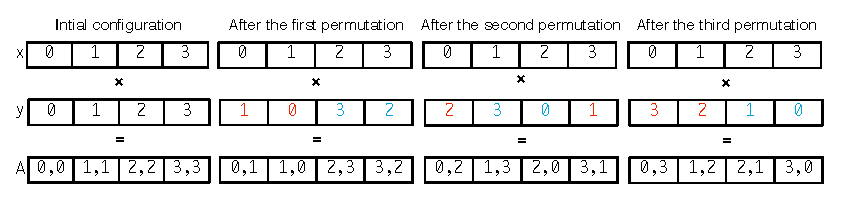
\includegraphics[scale=0.6]{lowlevelopt/pictures/vect-by-vect-inline.pdf}}
\caption{The outer-product vectorization relies on permuting values directly within vector registers.}
\label{fig:vect-by-vect}
\end{figure}

The storage layout of {\tt PA}, however, is incorrect after the application of this outer-product-based vectorization. It can be efficiently restored with a sequence of vector shuffles following the pattern highlighted in Figure~\ref{fig:restore-layout}, executed once outside of the \texttt{ijk} loop nest. The pseudo-code for the transformed weighted Laplace assembly kernel is shown in Listing~\ref{code:weighted-laplace-opvect}.

\begin{figure}[h]
\centerline{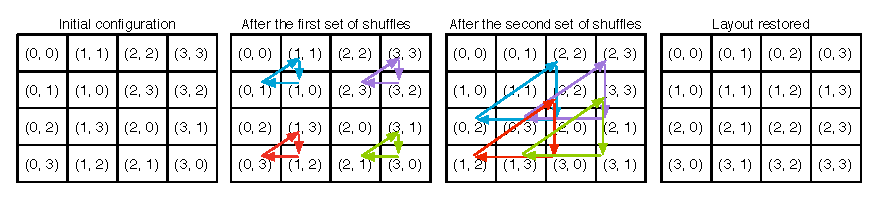
\includegraphics[scale=0.6]{lowlevelopt/pictures/vect-restore-inline.pdf}}
\caption{Restoring the storage layout is the last step of the outer-product vectorization. The figure shows how 4$\times$4 elements in the top-left block of the element matrix {\tt A} can be moved to their correct positions. Each rotation, represented by a group of three same-colored arrows, is implemented by a single shuffle intrinsic.}
\label{fig:restore-layout}
\end{figure}

\paragraph{Generalization}
In this section, we have considered assembly kernels arising from bilinear forms. The transformation can be generalized to linear forms provided that the loop over mesh elements is introduced in the computational model. The new dimension would induce an outer product with the test functions loop; hence, the element vector could be turned into a ``multi-element'' matrix, which would enable a similar vector-register tiling. This is however not implemented in COFFEE.

\section{Experiments}
\label{sec:coffee-perfeval}
The objective is to evaluate the impact of the code transformations presented in the previous sections in representative problems.

\subsection{Setup}
We use three bilinear forms, which we refer to as (i) {\tt Helmholtz}, (ii) {\tt Diffusion}, and (iii) {\tt Burgers} (the names derive from the PDEs from which the bilinear forms were extracted). The three chosen forms lead to \emph{real-life kernels} and comprise the core differential operators in some of the most frequently encountered finite element problems in scientific computing. This is of crucial importance because distinct problems, possibly arising in completely different fields, may employ (subsets of) the same differential operators of our benchmarks, which implies similarities and redundant patterns in the generated code. Consequently, the proposed code transformations have a domain of applicability that goes far beyond that of the three analyzed equations.

The {\tt Helmholtz} and {\tt Diffusion} kernels are archetypal second order elliptic operators. They are complete and unsimplified examples of the operators used to model diffusion and viscosity in fluids, and for imposing pressure in compressible fluids. As such, they are both extensively used in climate and ocean modeling. Very similar operators, for which the same optimisations are expected to be equally effective, apply to elasticity problems, which are at the base of computational structural mechanics. The {\tt Burgers} kernel is a typical example of a first order hyperbolic conservation law, which occurs in real applications whenever a quantity is transported by a fluid (the momentum itself, in our case). We chose this particular kernel since it applies to a vector-valued quantity, while the elliptic operators apply to scalar quantities; this impacts the generated code, as explained next. The operators we have selected are characteristic of both the second and first order operators that dominate fluids and solids simulations.

The benchmarks were written in UFL (code available at~\citep{ufl-code-lowlevelopt}) and executed over real unstructured meshes through Firedrake. The transformations are applied through COFFEE, which is used by Firedrake. The {\tt Diffusion} code has already been shown in Listing~\ref{code:weighted-laplace}. The {\tt Helmholtz} equation uses the same differential operators as {\tt Diffusion}. In the {\tt Helmholtz} kernel code, the main differences with respect to {\tt Helmholtz} are the presence of additional arrays (the basis functions for the ``mass term'') and constants for computing the element matrix. {\tt Burgers} is a non-linear problem employing differential operators different from those of {\tt Helmholtz} and relying on vector-valued quantities, which has a major impact on the generated assembly code (see Listing~\ref{code:burgers}), where a larger number of basis function arrays ($X1$, $X2$, ...) and constants ($F0$, $F1$, ..., $K0$, $K1$,...) are generated.

These problems were studied varying both the shape of mesh elements and the polynomial order $q$ of the function spaces, whereas the element family, Lagrange, is fixed. As might be expected, the larger the element shape and $q$, the larger the iteration space. Triangles, tetrahedra, and prisms were tested as element shape. For instance, in the case of {\tt Helmholtz} with $q=1$, the size of the \texttt{j} and \texttt{k} loops for the three element shapes is, respectively, $3$, $4$, and $6$. Moving to larger shapes has the effect of increasing the number of basis function arrays, since, intuitively, the behaviour of the equation has to be approximated also along a third axis. On the other hand, the polynomial order affects only the problem size (the three loops \texttt{i}, \texttt{j}, and \texttt{k}, and, as a consequence, the size of $X$ and $Y$ arrays). A range of polynomial orders from $q=1$ to $q=4$ were tested; higher polynomial orders are excluded from the study because of current Firedrake limitations. In all these cases, the size of the element matrix rarely exceeds 30$\times$30, with a peak of 105$\times$105 in {\tt Burgers} with prisms and $q=4$.

\subsection{Test Environment}
The experiments were run on a single core of an Intel architecture, a Sandy Bridge I7-2600 CPU running at 3.4 GHz, with 32KB of L1 cache and 256KB of L2 cache). The \texttt{icc 13.1} compiler was used. The compilation flags used were \texttt{-O2} and \texttt{-xAVX} for auto-vectorization (other optimization levels were tried, but they generally resulted in higher execution times). 

The execution times are the average of three runs with ``warm cache''; that is, with all kernels retrieved directly from the Firedrake's cache, so code generation and compilation times are not counted. The timing includes the costs of both matrix insertion and mesh iteration. 

\subsection{Rationale of the Experimentation}
We evaluate the impact of four transformations: generalized loop-invariant code motion (\emph{licm}); padding and data alignment (\emph{ap}); outer-product vectorization (\emph{op-vect}); expression splitting (\emph{split}). We also study \emph{licm}, despite not considering it a real low level transformation (it is actually a rewrite operator, see Chapters~\ref{ch:optimality} and~\ref{ch:coffee}), because measuring the impact of \emph{ap}, \emph{op-vect}, and \emph{split} becomes realistic only when all additional loops and temporaries have been created.

Figure~\ref{fig:coffee-individual-res} shows the maximum speed-ups achieved by composing the four transformations over the original code generated by Firedrake via the FEniCS Form Compiler. The figure is a three-dimensional plot: each subplot is a specific ${\langle} \textrm{shape}, \mathrm{form}, q {\rangle}$ problem instance, with $q$ varying within each subplot. By referring to this figure, in the next sections we motivate the performance improvements obtained.

\begin{figure}[t]
\centerline{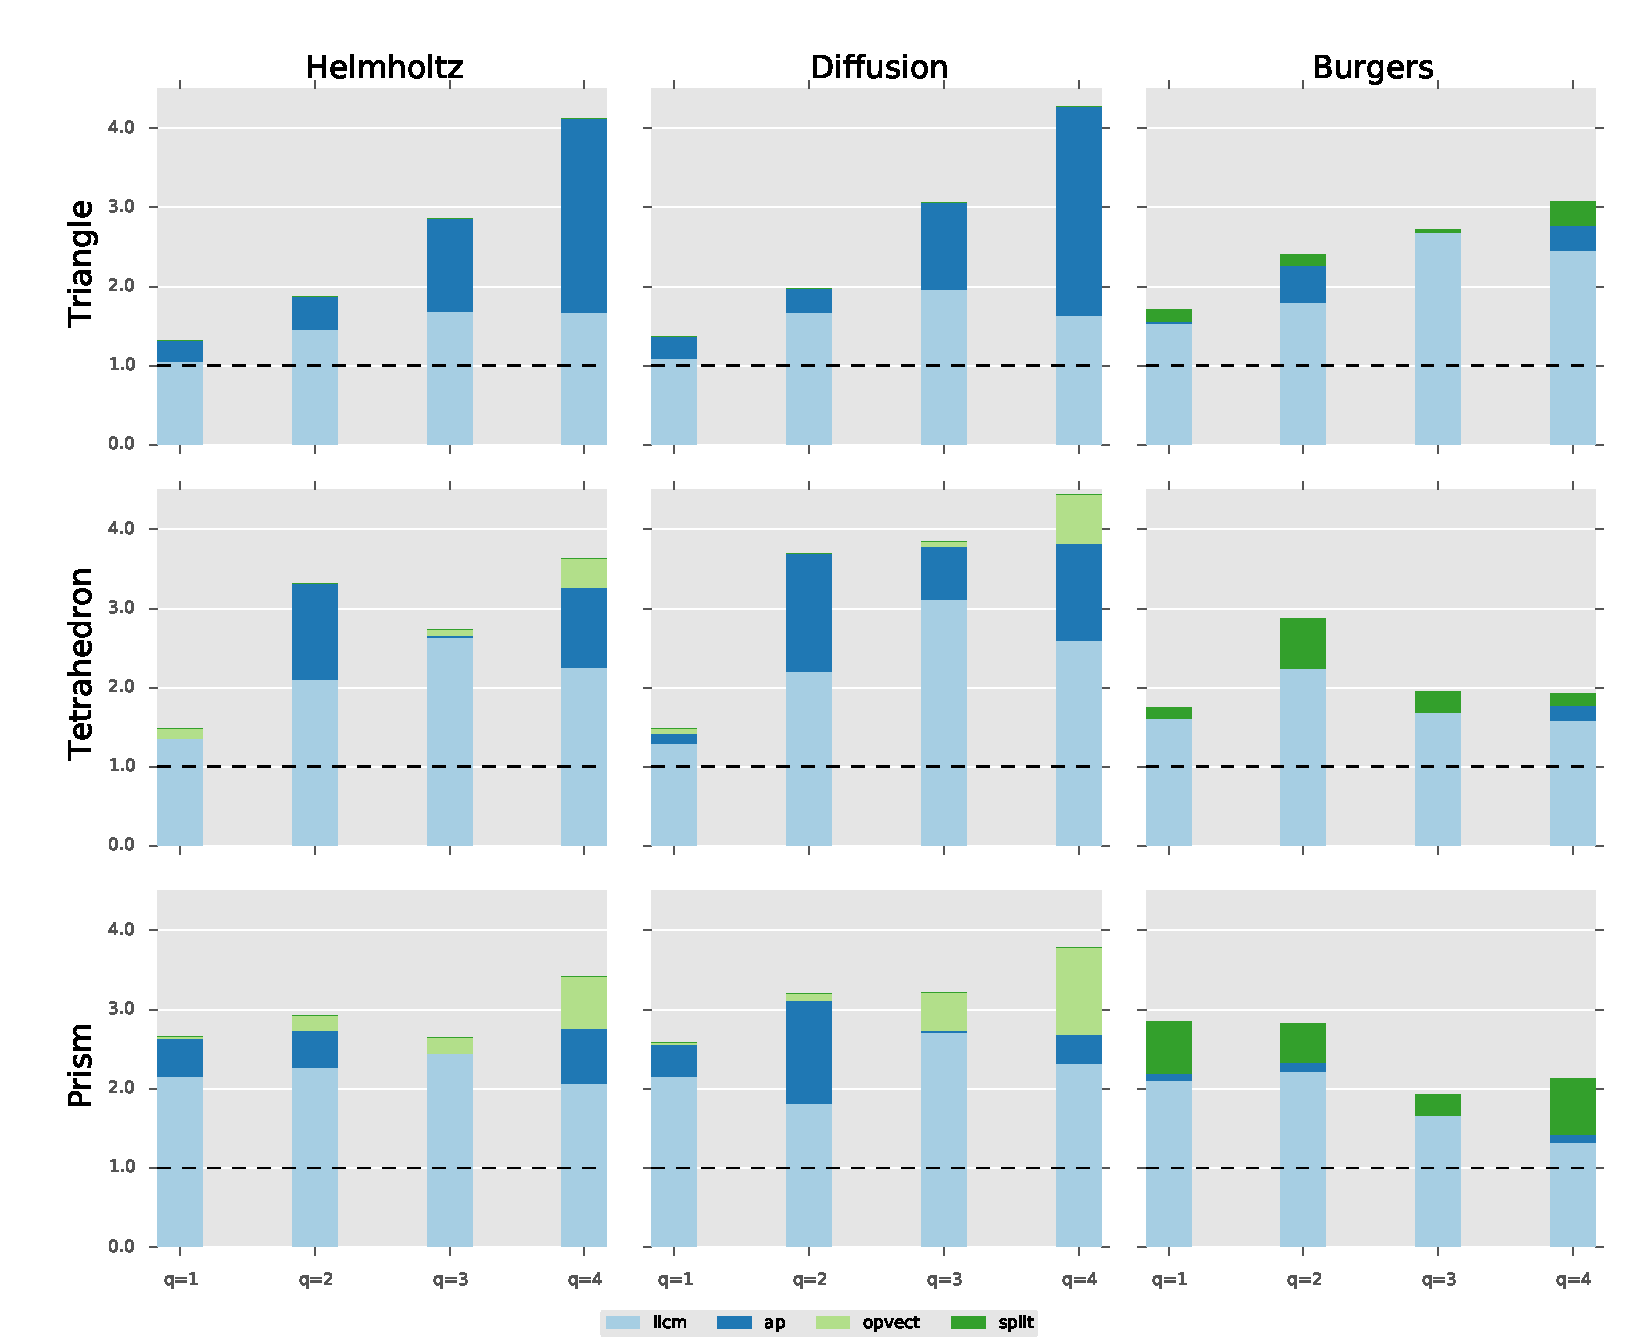
\includegraphics[scale=0.45]{lowlevelopt/perf-results/individual/plot_sb}}
\caption{Maximum performance improvement on a Sandy Bridge due to generalized loop-invariant code motion, padding and data alignment, outer-product vectorization, and expression splitting over the original code produced by Firedrake. The unroll and splitting factors -- respectively for the outer-product vectorization and expression splitting -- were determined empirically.}
\label{fig:coffee-individual-res}
\end{figure}


\subsubsection{Impact of Generalized Loop-invariant Code Motion}
\label{sec:perf-eval-licm}

In general, the speed-ups achieved by \emph{licm} are notable, which is in line with what we have observed in Chapter~\ref{ch:optimality}. The main reasons are that in the original code, (i) sub-expressions invariant to outer loops are not automatically hoisted, while (ii) sub-expressions invariant to the innermost loop are hoisted, but their execution is not auto-vectorized. These observations derive from inspection of assembly code generated by the compiler. 

The gain tends to grow with the computational cost of the kernels: bigger loop nests (i.e., larger element shapes and polynomial orders) usually benefit from the reduction in redundant computation, even though extra memory for the temporary arrays is required. Some discrepancies to this trend are due to a less effective auto-vectorization. For instance, on the Sandy Bridge, the improvement at $q=3$ is larger than that at $q=4$ because, in the latter case, the size of the innermost loop is not a multiple of the vector length, and a remainder scalar loop is introduced at compile time. Since the loop nest is small, the cost of executing the extra scalar iterations can have a significant impact.

\subsubsection{Impact of Padding and Data Alignment}
\label{sec:perf-eval-padding}

Padding, which avoids the introduction of a remainder loop as described in Section~\ref{sec:coffee-padding}, as well as data alignment, enhance the quality of auto-vectorization. Occasionally the impact of \emph{ap} is marginal. These may be due to two reasons: (i) the non-padded element tensor size is already a multiple of the vector length; (ii) the number of aligned temporaries introduced by \emph{licm} is so large to induce cache associativity conflicts (e.g. {\tt Burgers}).

\subsubsection{Impact of Vector-register Tiling}
\label{sec:perf-eval-opvect}

\emph{op-vect} requires setting an unroll-and-jam factor. Here, we discuss the speed-ups obtained after a small set of feasible unroll-and-jam factors (between 1 and 4) were tried (i.e., the maximum speed-ups). 

The rationale behind these results is that the effect of \emph{op-vect} is significant in problems in which the assembly loop nest is relatively big. When the loops are short, since the number of arrays accessed at every loop iteration is rather small (between 4 and 8 temporaries, plus the element matrix itself), there is no need for
vector-register tiling; extensive unrolling is sufficient to improve register re-use and, therefore, to maximize the performance. However, as the iteration space becomes larger, \emph{op-vect} leads to improvements up to 1.4$\times$ ({\tt Diffusion}, prismatic mesh, $q=4$ - increasing the overall speed up from 2.69$\times$ to 3.87$\times$).

Using the Intel Architecture Code Analyzer tool~\citep{IACA}, we confirmed that speed ups are a consequence of increased register re-use. In {\tt Helmholtz} $q=4$, for example, the tool showed that when using \emph{op-vect} the number of clock cycles to execute one iteration of the \texttt{j} loop decreases by roughly 17$\%$, and that this is a result of the relieved pressure on both of the data (cache) ports available in the core.

The performance of individual kernels in terms of floating-point operations per second was also measured. The theoretical peak on a single core, with the Intel Turbo Boost technology activated, is 30.4 GFlop/s. In the case of {\tt Diffusion} using a prismatic mesh and $q=4$, we achieved a maximum of 21.9 GFlop/s with \emph{op-vect} enabled, whereas 16.4 GFlop/s was obtained when only \emph{licm} and \emph{ap} were used. This result is in line with the expectations: analysis of assembly code showed that, in the \texttt{jk} loop nest, which in this problem represents the bulk of the computation, 73$\%$ of instructions are actually floating-point operations.

Application of \emph{op-vect} to the {\tt Burgers} problem induces significant slowdowns due to the large number of temporary arrays that need be tiled, which exceeds the available logical registers on the underlying architecture. Expression splitting can be used in combination with \emph{op-vect} to alleviate this issue; this is discussed in the next section.

%for which efficient register allocation can be already guaranteed

\subsubsection{Impact of Expression Splitting}
\label{sec:perf-results-split} 
Expression splitting relieves the register pressure when the element matrix evaluation needs to read from a large number of basis function arrays. As detailed in Section~\ref{sec:coffee-split}, the price to pay for this optimization is an increased number of accesses to the element matrix and, potentially, redundant computation. 

For the {\tt Helmholtz} and {\tt Diffusion} kernels, in which only between 4 and 8 temporaries are read at every loop iteration, \texttt{split} tends to slow down the computation, because of the aforementioned drawbacks. Slow-downs up to 1.4$\times$ were observed. 

In the {\tt Burgers} kernels, between 12 and 24 temporaries are accessed at every loop iteration, so \emph{split} plays a key role since the number of available logical registers on the Sandy Bridge architecture is only 16. In almost all cases, a split factor of 1, meaning that the original expression was divided into two parts, ensured close-to-peak performance. The transformation negligibly affected register locality, so speed-ups up to 1.5$\times$ were observed. For instance, when $q=4$ and a prismatic mesh is employed, the overall performance improvement increases from 1.44$\times$ to 2.11$\times$. 

The performance of the {\tt Burgers} kernel on a prismatic mesh was 20.0 GFlop/s from $q=1$ to $q=3$, while it was 21.3 GFlop/s in the case of $q=4$. These values are notably close to the peak performance of 30.4 GFlop/s. Disabling \emph{split} makes the performance drop to 17.0 GFlop/s for $q=1, 2$, 18.2 GFlop/s for $q=3$, and 14.3 GFlop/s for $q=4$. These values are in line with the speed-ups shown in Figure~\ref{fig:coffee-individual-res}.

The \emph{split} transformation was also tried in combination with \emph{op-vect} (\emph{split-op-vect}). Despite improvements up to 1.22$\times$, \emph{split-op-vect} never outperforms \emph{split}. This is motivated by two factors: for small split factors, such as 1 and 2, the data space to be tiled is still too big, and register spilling affects run-time; for higher ones, sub-expressions become so small that, as explained in Section~\ref{sec:perf-eval-opvect}, extensive unrolling already allows to achieve a certain degree of register re-use.

\subsubsection{More Registers, Larger Vectors}
To assess the impact of the transformations on architectures with different numbers of vector registers and SIMD lanes, we have repeated the same experiments on an Intel Xeon Phi (5110P, running at 1.05Ghz in native mode, 32KB L1 cache and 512KB L2 cache). The \texttt{icc 13.1} compiler was used. The compilation flag used for optimization was \texttt{-O3}. 

As opposed to the Sandy Bridge, which only had 16 256-bit vector-registers, the Xeon Phi has 32 512-bit vector registers. Since our transformations focus on register locality and SIMD vectorization, it is useful to study such a different platform. 

The results of the experimentation are presented in Figure~\ref{fig:coffee-individual-res-phi}. Overall, the trend is similar to that observed on the Sandy Bridge, with a few exceptions. {\em licm} is occasionally inconsequential because the remainder loop overhead is more pronounced on the Xeon Phi, where the vector length is twice as long, which leads to proportionately larger fractions of scalar code. The pattern of {\em ap} and {\em op-vect}, instead, is much more similar to the one on the Sandy Bridge (higher speed-ups were often observed). The impact of {\em split} in {\tt Burgers} is not as pronounced as on the Sandy Bridge, since register spilling is now limited by the presence of 32 logical vector units. 

\begin{figure}[t]
\centerline{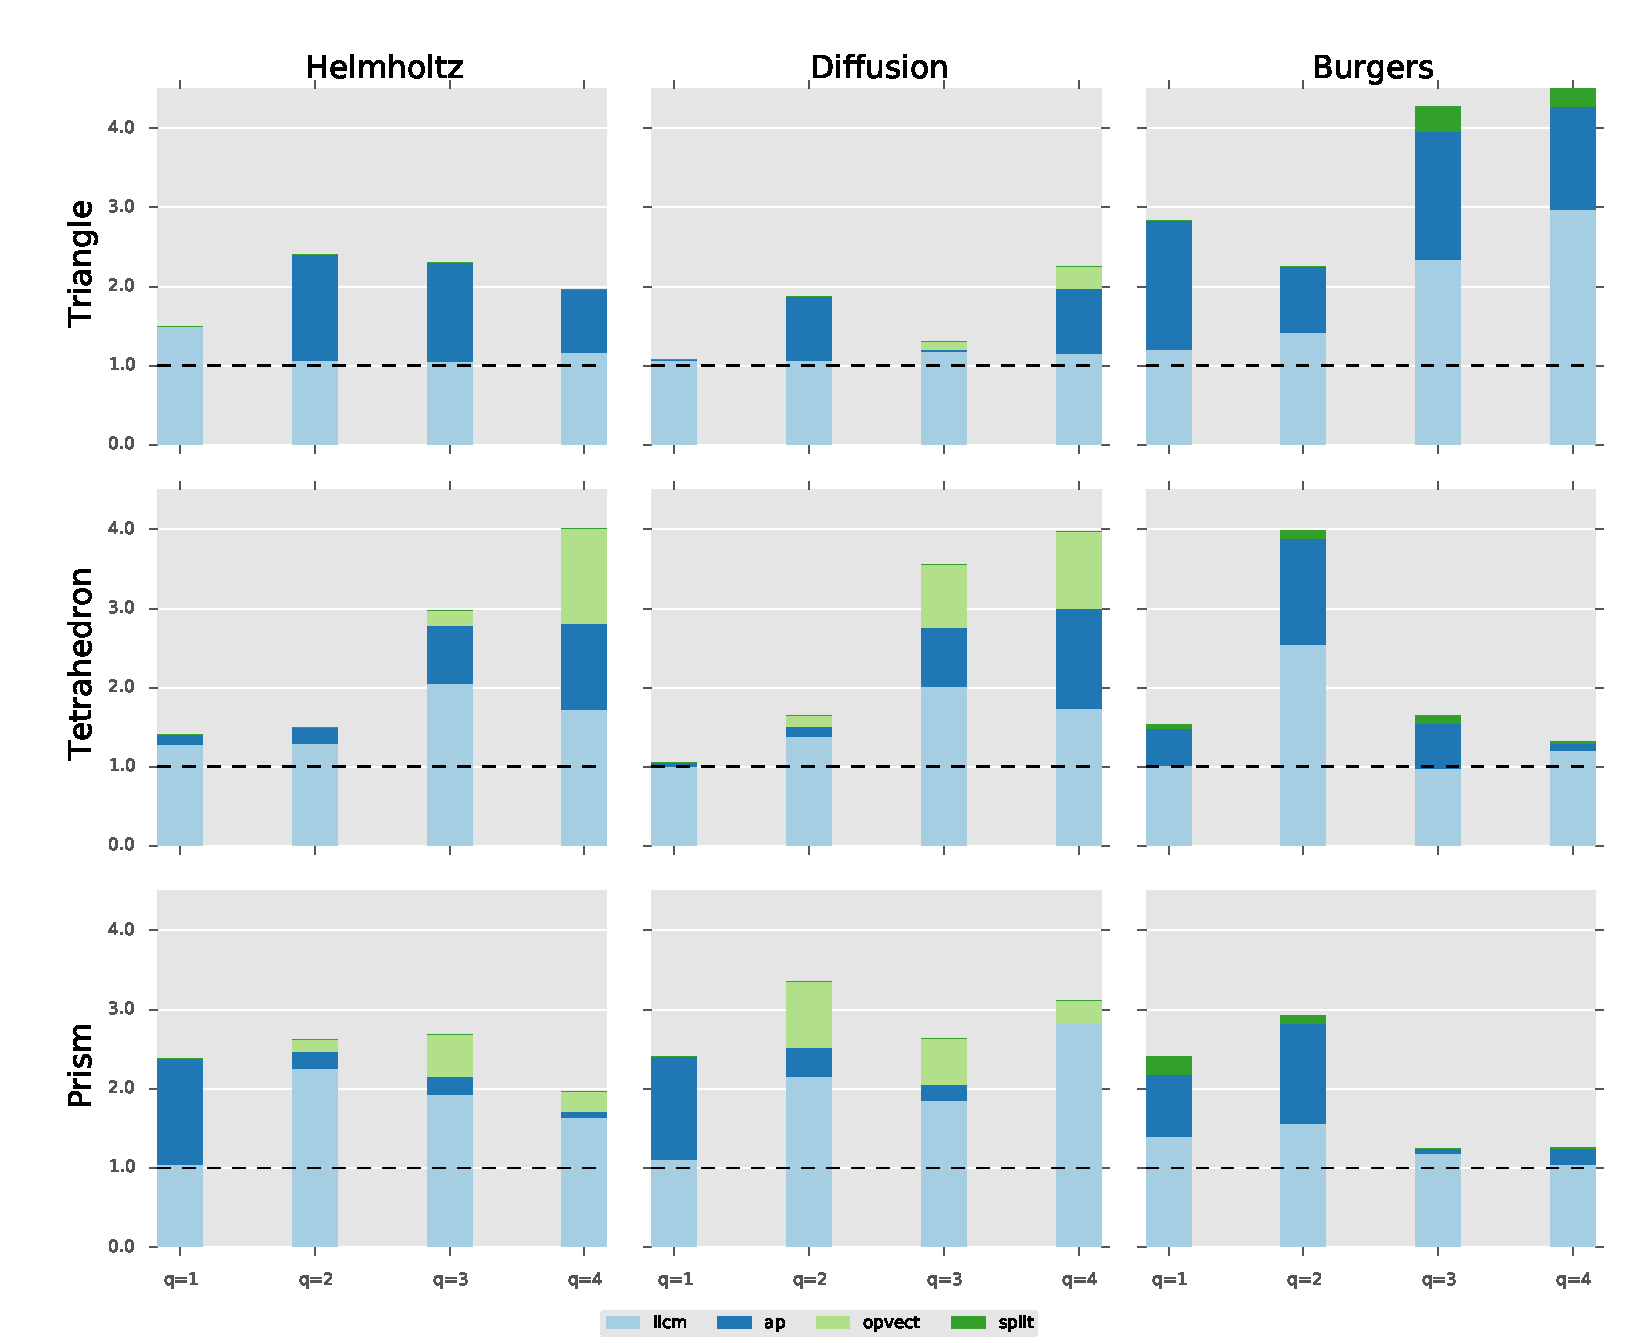
\includegraphics[scale=0.45]{lowlevelopt/perf-results/individual/plot_phi}}
\caption{Maximum performance improvement on a Xeon Phi due to generalized loop-invariant code motion, padding and data alignment, outer-product vectorization, and expression splitting over the original code produced by Firedrake. The unroll and splitting factors -- respectively for the outer-product vectorization and expression splitting -- were determined empirically.}
\label{fig:coffee-individual-res-phi}
\end{figure}


\subsubsection{Summary of Results}
We have analyzed the impact of three low level optimizations on top of {\em licm}. While {\em ap} is demonstrated to provide systematic improvements, the impact of {\em op-vect} and {\em split} is more difficult to predict. {\em op-vect} requires relatively large loop nests (the trip count of individual loops must be at least larger than 10) to be effective, as observed in {\tt Helmholtz} and {\tt Diffusion}. The largest gains in {\tt Burgers} derive from using {\em split}, because of the high register pressure. Composing {\em op-vect} and {\em split} in {\tt Burgers} rarely provided benefits, and most of these were significantly smaller than those achieved through {\tt ap}. This was verified on both the Sandy Bridge and the Xeon Phi. It is unclear why on the Xeon Phi, in spite of a larger number of vector registers, the composite {\em split-op-vect} transformation did not result in significant performance improvements.

These results suggest that a cost model or an auto-tuning system to select the optimal composite transformation for a given problem would be of great help. We expand on this problem in Section~\ref{sec:coffee-related-work}.

\section{Experience with Traditional Compiler Optimizations}
\label{sec:coffee-genpurp-opts}
In this section, we report on an experimentation with traditional optimizations: loop interchange, loop unroll, vector promotion and loop fusion. The following sections also discuss the implementation and the use of these transformations in COFFEE. 

\subsection{Loop Interchange}
\label{sec:coffee-genpurp-opts-interchange}
All loops are interchangeable, provided that temporaries are introduced if the nest is not perfect. For the employed storage layout, the loop permutations \texttt{ijk} and \texttt{ikj} are likely to maximize the performance. Conceptually, this is motivated by the fact that if the \texttt{i} loop were in an inner position, then a significantly higher number of load instructions would be required at every iteration. We tested this hypothesis in manually crafted kernels. We found that the performance loss is greater than the gain due to the possibility of accumulating increments in a register, rather than memory, along the \texttt{i} loop. The choice between \texttt{ijk} and \texttt{ikj} depends on the number of load instructions that can be hoisted out of the innermost dimension. A good heuristics is to choose as outermost the loop along which the number of invariant loads is smaller so that more registers remain available to carry out the computation of the element tensor. 

Our experience with the Intel and GNU compilers is controversial: if, on one hand, the former applies this transformation following a reasonable cost model, the latter is generally too conservative, even at highest optimization level. This behaviour was verified in different variational forms (by looking at assembly code and compiler reports), including the complex hyperelastic model analyzed in Chapter~\ref{ch:optimality}. 

Loop interchange is implemented in COFFEE. However, it is not applied by any of the default optimization levels (see Section~\ref{sec:coffee:pipeline}) due to the lack of a cost model capable of providing systematic performance improvements across a range of problems and general-purpose compilers.  

\subsection{Loop Unroll}
We first observe that manual full (or extensive) unrolling is unlikely to be effective for two reasons. Firstly, the \texttt{ijk} loop nest would need to be small enough such that the unrolled instructions do not exceed the instruction cache, which is rarely the case: it is true that in a local assembly kernel the minimum size of the \texttt{ijk} loop nest is 3$\times$3$\times$3 (triangular mesh and polynomial order 1), but this increases rapidly with the polynomial order of the method and the discretization employed (e.g. tetrahedral meshes imply larger loop nests than triangular ones), so sizes greater than 10$\times$10$\times$10, for which extensive unrolling would already be harmful, are in practice very common. Secondly, manual unrolling is dangerous because it may compromise compiler auto-vectorization by either removing loops (most compilers search for vectorizable loops) or losing spatial locality within a vector register.

By comparison to implementations with manually-unrolled loops, we noticed that recent versions of compilers like GNU's and Intel's estimate close-to-optimal unroll factors when the loops are affine and their bounds are relatively small and known at compile-time, which is the case of our kernels. Our choice, therefore, is to relieve COFFEE from the duty of applying loop fusion and to leave the back-end compiler in charge of selecting unroll factors.

\subsection{Vector promotion}
\label{sec:coffee-precompute}
Vector promotion is a transformation that ``trades'' a parallel dimension for space, thus creating SIMD vectorization opportunities for outer loops. In this section, we consider vector promotion for the sub-expressions that only depend on the integration loop (i.e., the {\tt i} loop). 

\begin{algorithm}
\scriptsize\ttfamily
\SetAlgorithmName{LISTING}{}
\KwSty{void} weighted$\_$laplace(\KwSty{double} A[3][3], \KwSty{double} **coords, \KwSty{double} w[3]) $\lbrace$\\
~~// Omitting redundant code \\
~~...\\
~~// Application of vector promotion
~~\KwSty{double} f0[6] = $\lbrace$0.0$\rbrace$;\\
~~\KwSty{for} (\KwSty{int} i = 0; i$<$6; i++) $\lbrace$ \\
~~~~\KwSty{for} (\KwSty{int} r  = 0; r < 3; ++r) $\lbrace$ \\
~~~~~~f0[i] += (w[r] * C[i][r]);\\
~~~~$\rbrace$ \\
~~$\rbrace$\\
~~\KwSty{for} (\KwSty{int} i = 0; i$<$6; i++) $\lbrace$ \\
~~~~\KwSty{double} T0[3];\\
~~~~\KwSty{double} T1[3];\\
~~~~\KwSty{for} (\KwSty{int} j = 0; j$<$3; j++) $\lbrace$ \\
~~~~~~T0[j] = ((K[1]*B[i][j])+(K[3]*D[i][j]));\\
~~~~~~T1[j] = ((K[0]*B[i][j])+(K[2]*D[i][j]));\\
~~~~$\rbrace$\\
~~~~\KwSty{double} T2[3];\\
~~~~\KwSty{double} T3[3];\\
~~~~\KwSty{for} (\KwSty{int} k = 0; k$<$3; k++) $\lbrace$ \\
~~~~~~T2[k] = ((K[1]*B[i][k])+(K[3]*D[i][k]));\\
~~~~~~T3[k] = ((K[0]*B[i][k])+(K[2]*D[i][k]));\\
~~~~$\rbrace$\\
~~~~\KwSty{for} (\KwSty{int} j = 0; j$<$3; j++) $\lbrace$\\
~~~~~~\KwSty{for} (\KwSty{int} k = 0; k$<$3; k++) $\lbrace$\\
~~~~~~~~A[j][k] += (T0[j]*T2[k] + T1[j]*T3[k])*det*W[i]*f0[i]);\\
~~~~~~$\rbrace$\\
~~~~$\rbrace$\\
~~$\rbrace$\\
$\rbrace$

\caption{The assembly kernel for the weighted Laplace operator in Listing~\ref{code:weighted-laplace} after application of vector promotion on top of generalized code motion.}
\label{code:weighted-laplace-vector-prom}
\end{algorithm}

In Listing~\ref{code:weighted-laplace-vector-prom}, the evaluation of the coefficient \texttt{w} on the basis functions in {\tt C} is made vectorizable along the {\tt i} loop by ``promoting'' the scalar \texttt{f} to an array of size 6. All sub-expressions hoisted at the level of the {\tt i} loop (which result from applying the techniques described in Chapter~\ref{ch:optimality}) can be treated similarly. The cost of this transformation obviously depends on the amount of computation within the {\tt i} loop: the larger the number of scalars to be turned into arrays, the bigger the resulting working set, which may lead to the same memory issues explained in Section~\ref{sec:mem-const}. Loop tiling may be used to counteract this effect, but the implementation complexity would be significantly higher. 

Neither the GNU nor the Intel compiler seems capable of applying this transformations, probably because of the non-trivial impact on the working set. In fact, it is challenging to propose a cost model that works well even just for the class of assembly kernels considered in this chapter. Vector promotion is implemented in COFFEE, but unused by any of the default optimization pipelines. 

\subsection{Loop Fusion}
\label{sec:coffee-loopfusion}

In assembly kernels arising from bilinear forms, test and trial functions may belong to the same function space. Further, the same subset of operators is sometimes applied to both sets of functions. In such a case, not only do the {\tt j} and {\tt k} loops have same trip count, but also sub-expressions that differ in just the {\tt j} and {\tt k} array indices appear. We refer to these as ``almost common sub-expressions''. The clone loops created by generalized loop-invariant code motion can easily be fused (they have the same size and no data dependencies  are present) and the redundant computation induced by the almost common sub-expressions be avoided. The result of this transformation can be observed by comparing Listing~\ref{code:weighted-laplace-loopfusion} to some of the previous code snippets, for instance Listing~\ref{code:weighted-laplace-licm-pad}.

\begin{algorithm}
\scriptsize\ttfamily
\SetAlgorithmName{LISTING}{}
\KwSty{void} weighted$\_$laplace(\KwSty{double} A[3][3], \KwSty{double} **coords, \KwSty{double} w[3]) $\lbrace$\\
~~// Omitting redundant code \\
~~...\\
~~\KwSty{for} (\KwSty{int} i = 0; i$<$6; i++) $\lbrace$ \\
~~~~\KwSty{double} f0  = 0.0;\\
~~~~\KwSty{for} (\KwSty{int} r  = 0; r < 3; ++r) $\lbrace$ \\
~~~~~~f0 += (w[r] * C[i][r]);\\
~~~~$\rbrace$ \\
~~~~\KwSty{double} T0[3];\\
~~~~\KwSty{double} T1[3];\\
~~~~// Fused loop with almost common sub-expressions detected\\
~~~~\KwSty{for} (\KwSty{int} r = 0; r$<$3; r++) $\lbrace$ \\
~~~~~~T0[r] = ((K[1]*B[i][r])+(K[3]*D[i][r]));\\
~~~~~~T1[r] = ((K[0]*B[i][r])+(K[2]*D[i][r]));\\
~~~~$\rbrace$\\
~~~~\KwSty{for} (\KwSty{int} j = 0; j$<$3; j++) $\lbrace$\\
~~~~~~\KwSty{for} (\KwSty{int} k = 0; k$<$3; k++) $\lbrace$\\
~~~~~~~~A[j][k] += (T0[j]*T0[k] + T1[j]*T1[k])*det*W[i]*f0);\\
~~~~~~$\rbrace$\\
~~~~$\rbrace$\\
~~$\rbrace$\\
$\rbrace$\\
\caption{The assembly kernel for the weighted Laplace operator in Listing~\ref{code:weighted-laplace} after application of loop fusion on top of generalized code motion.}
\label{code:weighted-laplace-loopfusion}
\end{algorithm}

Although loop fusion is applicable by most general-purpose compilers, the detection of almost common sub-expressions is not. There are several possible explanations for this, including: the transformation is of domain-specific nature; common sub-expressions elimination occurs at an earlier stage in the optimization pipeline; common sub-expressions elimination cannot distinguish different loop indices (i.e., it cannot detect almost common sub-expressions). We have therefore implemented this special version of loop fusion in COFFEE, with satisfactory results. In our experiments, this transformations results in relatively small performance improvements, ranging between $2\%$ and $7\%$. The speed-ups, however, are systematic across different forms, discretizations and general-purpose compilers, so loop fusion is performed automatically in the optimization process. This is elaborated in Chapter~\ref{ch:coffee}.

\section{Related Work}
\label{sec:coffee-related-work}
The code transformations presented in Section~\ref{sec:lowlevelopt} are inspired by standard compiler optimizations and by the structure of the assembly kernels. Expression splitting is an abstract variant of loop fission based on properties of arithmetic operators. The outer-product vectorization is an implementation of tiling at the level of vector registers; tiling, or ``loop blocking'', is commonly used to improve data locality (especially for caches). Padding has been used to achieve data alignment and to improve the effectiveness of vectorization; the idea of changing the storage layout by adding ``ghost regions'' is however widespread. A standard reference for the compilation techniques re-adapted in this work is~\cite{dragonbook}.

Our compiler-based optimization approach is made possible by the top-level DSL, which enables automated code generation. DSLs have been proven successful in auto-generating optimized code for other domains: Spiral~\citep{Pueschel:05} for digital signal processing numerical algorithms, ~\citep{Spampinato:14} for dense linear algebra, or Pochoir~\citep{pochoir} and SDSL~\citep{stencil-compiler} for image processing and finite difference stencils. Similarly, PyOP2 is used by Firedrake to express iteration over unstructured meshes in scientific codes. COFFEE improves automated code generation in Firedrake.

In~\cite{Markall20101815}, the optimization of global assembly, rather than local assembly, has been treated for both CPUs and GPUs. \cite{petsc-integration-gpu} focus on improving the performance of assembly kernels on GPUs through efficient parallelization. In~\cite{assembly-opencl}, variants of the standard numerical integration algorithm have been specialized and evaluated for the PowerXCell processor. A standard reference for the optimization of both local and global assembly on GPUs is~\citep{fem-gpu-study}. All these studies, despite tackling low level optimization, lack an exhaustive study from the compiler viewpoint; in addition, none of them relies on automated code generation. The optimizations presented in Section~\ref{sec:lowlevelopt} are also never mentioned. 

COFFEE would benefit from a cost model or an auto-tuning system to select, for a given problem, the best combination of low level optimizations. This would relieve users from the burden of performance tuning. A cost model was introduced in~\cite{Luporini-coffee}, but in light of the achievements in Chapter~\ref{ch:optimality}, it now requires refinements to be effective. Many code generators, like those based on the Polyhedral model~\citep{pluto} and those driven by domain-knowledge~\citep{modeldriven}, make use of cost models. The alternative of using auto-tuning has been adopted by nek5000~\citep{nek5000} for small matrix-matrix multiplies, the ATLAS library~\citep{ATLAS}, FFTW~\citep{FFTW} for fast fourier transforms, Spiral \citep{Pueschel:05}, and LGen~\citep{Spampinato:14}. 


\section{Applicability to Other Domains}
\label{sec:generality}
We have demonstrated that our cross-loop optimizations for arithmetic intensity are effective in the context of automated code generation for finite element integration. In this section, we discuss their applicability in other computational domains and, more in general, their integrability within a general-purpose compiler.

There are neither conceptual nor technical reasons which prevent our transformations from being used in other (general-purpose, research, ...) compilers. It is challenging, however, to assess their potential in other computational domains. We here provide insights into this matter. The starting point of our work was the mathematical formulation of a finite element operator, expressible as:

\begin{equation}
\label{eq:assembly-model}
\scriptsize
\forall_{i, j} ~~~ A_{ij}^K = \sum_{q=1}^{n_1} \sum_{k=1}^{n_2} \alpha_{k, q}(a', b', c', ...) \beta_{q, i, j}(a, b, c, d, ...) \gamma_{q}(w_K, z_K)
\end{equation}

The expression represents the numerical evaluation of an integral at $n_1$ points in the mesh element $K$ computing the local element tensor $A$. Functions $\alpha$, $\beta$ and $\gamma$ are problem-specific and can be intricately complex, involving for example the evaluation of derivatives. We can however abstract from the structure of $\alpha$, $\beta$ and $\gamma$ to highlight a number of aspects

\begin{description}
\item[Optimizing mathematical expressions] Expression manipulation (e.g. simplification, decomposition into sub-expressions) opens multiple semantically equivalent code generation opportunities, characterized by different trade-offs in parallelism, redundant computation, and data locality. The basic idea is to exploit properties of arithmetic operators, such as associativity and commutativity, to re-schedule the computation suitably for the underlying architecture. Loop-invariant code motion and expression splitting follow this principle, so they can be re-adapted or extended to any domains involving numerical evaluation of complex mathematical expressions (e.g. electronic structure calculations in physics and quantum chemistry relying on tensor contractions, which we reviewed in Section~\ref{sec:bkg:tce}). In this context, we highlight three points.
\begin{enumerate}
\item In~\eqref{eq:assembly-model}, the summations correspond to reduction loops, whereas loops over indices $i$ and $j$ are fully parallel. In our computational model, a kernel is executed by a single thread, which is likely to be the best strategy for standard multi-core CPUs. On the other hand, we note that for certain architectures (for example GPUs) this could be prohibitive due to memory requirements. Intra-kernel parallelization is one possible solution: a domain-specific compiler could map mathematical quantifiers and operators to different parallelization schemes and generate distinct variants of multi-threaded kernel code. Based on our experience, we believe this approach is necessary for achieving performance portability.
\item The various sub-expressions in $\beta$ only depend on (i.e. iterate along) a subset of the enclosing loops. In addition, some of these sub-expressions might reduce to the same values as iterating along certain iteration spaces. This code structure motivated the generalized loop-invariant code motion technique. The intuition is that whenever sub-expressions invariant with respect to different sets of affine loops can be identified, the question of whether, where and how to hoist them, while minimizing redundant computation, arises. Vector promotion also increases memory requirements due to the need for temporary arrays, so it is possible that for certain architectures the transformation could actually cause slow-downs (e.g. whenever the available per-core memory is small).
\item Associative arithmetic operators are the prerequisite for expression splitting. In essence, this transformation concerns resource-aware execution. In our context, expression splitting has been applied to improve register pressure. However, the underlying idea of re-scheduling (re-associating) operations to optimize for some generic parameters is far more general. It could be used, for example, as a starting point to perform kernel fission; that is, splitting a kernel into multiple parts, each part characterized by less stringent memory requirements (a variant of this idea for non-affine loops in unstructured mesh applications has been adopted in~\cite{op2-lcpc}). In~\eqref{eq:assembly-model}, for instance, not only can any of the functions $\alpha$, $\beta$ and $\gamma$ be split (assuming they include associative operators), but $\alpha$ could be completely extracted and evaluated in a separate kernel. This would reduce the working set size of each of the kernel functions, an option which is particularly attractive for many-core architectures in which the available per-core memory is much smaller than that in traditional CPUs.
\end{enumerate}
\item[Code generation and applicability of the transformations] All array sizes and loop bounds, for example $n_1$ and $n_2$ in~\eqref{eq:assembly-model}, are known at code generation time. This means that ``good'' code can be generated. For example, loop bounds can be made explicit, arrays can be statically initialized, and pointer aliasing is easily avoidable. Further, all of these factors contribute to the applicability and the effectiveness of some of our code transformations. For instance, knowing loop bounds allows both generation of correct code when applying vector-register tiling and discovery of redundant computation  opportunities. Padding and data alignment are special cases, since they could be performed at run-time if some values were not known at code generation time. Theoretically, they could also be automated by a general-purpose compiler through profile-guided optimization, provided that some sort of data-flow analysis is performed to ensure that the extra loop iterations over the padded region do not affect the numerical results. 
\item[Multi-loop vectorization] Compiler auto-vectorization has become increasingly effective in a variety of codes. However, multi-loop vectorization involving the loading and storing of data along a subset of the loops characterizing the iteration space (rather than just along the innermost loop), is not supported by available general-purpose compilers. The outer-product vectorization technique presented in this chapter shows that two-loop vectorization can outperform standard auto-vectorization. In addition, we expect the performance gain to scale with the number of vectorized loops and the vector length (as demonstrated in  the Xeon Phi experiments). Although the automation of multi-loop vectorization in a general-purpose compiler is far from straightforward, especially if stencils are present, we believe that this could more easily be achieved in specific domains. The intuition is to map the memory access pattern onto vector registers, and then to exploit in-register shuffling to minimize the traffic between memory and processor. By demonstrating the effectiveness of multi-loop vectorization in a real scenario, our research represents an incentive towards a systematic study of this technique.
\end{description}

\section{Conclusions}
\label{sec:coffee-conclusion}
In this chapter, we have presented the study and systematic performance evaluation of a class of composable cross-loop optimizations for improving arithmetic intensity in finite element local assembly kernels. In the context of automated code generation for finite element local assembly, COFFEE is the first compiler capable of introducing low-level optimizations to simultaneously maximize register locality and SIMD vectorization. Assembly kernels have particular computational characteristics. Their iteration space is usually very small, with the size depending on aspects like the degree of accuracy one wants to reach (polynomial order of the method) and the mesh discretization employed. The data space, in terms of number of arrays and scalars required to evaluate the element tensor, grows proportionally with the complexity of the finite element problem. The various optimizations overcome limitations of current vendor and research compilers. The exploitation of domain knowledge allows some of them to be particularly effective, as demonstrated by our experiments on a state-of-the-art Intel platform. The generality and the applicability of the proposed code transformations to other domains has also been discussed.
